\documentclass[12pt,utf8,notheorems,compress,t,aspectratio=169]{beamer}
%\documentclass[12pt,utf8,notheorems,compress,t]{beamer}
\usepackage{etex}

\usepackage{pgfpages}
\usepackage[export]{adjustbox}

% Workaround for the issue described at
% https://tex.stackexchange.com/questions/164406/beamer-using-href-in-notes.
\newcommand{\fixedhref}[2]{\makebox[0pt][l]{\hspace*{\paperwidth}\href{#1}{#2}}\href{#1}{#2}}

\usepackage[english]{babel}

\usepackage[normalem]{ulem}
\usepackage{graphbox}
\usepackage{mathtools}
\usepackage{booktabs}
\usepackage{stmaryrd}
\usepackage{amssymb}
\usepackage{manfnt}
\usepackage{array}
\usepackage{ragged2e}
\usepackage{multicol}
\usepackage{tabto}
\usepackage{xstring}
\usepackage{proof}
\usepackage{ifthen}
\usepackage[normalem]{ulem}
\usepackage[all]{xy}
\xyoption{rotate}
\usepackage{tikz}
\usetikzlibrary{calc,shapes,shapes.callouts,shapes.arrows,patterns,fit,backgrounds,decorations.pathmorphing,positioning,svg.path}
\hypersetup{colorlinks=true}

\newcommand*\circled[1]{\tikz[baseline=(char.base)]{%
  \node[shape=circle,draw,inner sep=1pt] (char) {#1};}}

\DeclareFontFamily{U}{bbm}{}
\DeclareFontShape{U}{bbm}{m}{n}
   {  <5> <6> <7> <8> <9> <10> <12> gen * bbm
      <10.95> bbm10%
      <14.4>  bbm12%
      <17.28><20.74><24.88> bbm17}{}
\DeclareFontShape{U}{bbm}{m}{sl}
   {  <5> <6> <7> bbmsl8%
      <8> <9> <10> <12> gen * bbmsl
      <10.95> bbmsl10%
      <14.4> <17.28> <20.74> <24.88> bbmsl12}{}
\DeclareFontShape{U}{bbm}{bx}{n}
   {  <5> <6> <7> <8> <9> <10> <12> gen * bbmbx
      <10.95> bbmbx10%
      <14.4> <17.28> <20.74> <24.88> bbmbx12}{}
\DeclareFontShape{U}{bbm}{bx}{sl}
   {  <5> <6> <7> <8> <9> <10> <10.95> <12> <14.4> <17.28>%
      <20.74> <24.88> bbmbxsl10}{}
\DeclareFontShape{U}{bbm}{b}{n}
   {  <5> <6> <7> <8> <9> <10> <10.95> <12> <14.4> <17.28>%
      <20.74> <24.88> bbmb10}{}
\DeclareMathAlphabet{\mathbbm}{U}{bbm}{m}{n}
\SetMathAlphabet\mathbbm{bold}{U}{bbm}{bx}{n}

\usepackage{pifont}
\newcommand{\cmark}{\ding{51}}
\newcommand{\xmark}{\ding{55}}
\DeclareSymbolFont{extraup}{U}{zavm}{m}{n}
\DeclareMathSymbol{\varheart}{\mathalpha}{extraup}{86}

\graphicspath{{images/}}

\usepackage[protrusion=true,expansion=true]{microtype}

\setlength\parskip{\medskipamount}
\setlength\parindent{0pt}

\title{Constructive forcing}

\author{Ingo Blechschmidt}
\date{September 20th to September 16th, 2023}

%\useinnertheme[shadow=true]
\setbeamerfont{block title}{size={}}

\useinnertheme{rectangles}

\usecolortheme{orchid}
\usecolortheme{seahorse}
\definecolor{mypurple}{RGB}{253,73,34}
\definecolor{mypurpledark}{RGB}{100,0,150}
\setbeamercolor{structure}{fg=mypurple}
\definecolor{myred}{RGB}{150,0,0}
%\setbeamercolor*{title}{bg=myred,fg=white}
%\setbeamercolor*{titlelike}{bg=myred,fg=white}
\setbeamercolor*{title}{bg=mypurple,fg=white}
\setbeamercolor*{titlelike}{bg=mypurple,fg=white}
\setbeamercolor{frame}{bg=black}

\usefonttheme{serif}
\usepackage[T1]{fontenc}
\usepackage{libertine}

% lifted from https://arxiv.org/abs/1506.08870
\DeclareFontFamily{U}{min}{}
\DeclareFontShape{U}{min}{m}{n}{<-> udmj30}{}
\newcommand\yon{\!\text{\usefont{U}{min}{m}{n}\symbol{'210}}\!}

\newcommand{\A}{\mathcal{A}}
\newcommand{\B}{\mathcal{B}}
\newcommand{\C}{\mathcal{C}}
\newcommand{\M}{\mathcal{M}}
\renewcommand{\AA}{\mathbb{A}}
\newcommand{\BB}{\mathbb{B}}
\newcommand{\pp}{\mathbbm{p}}
\newcommand{\MM}{\mathbb{M}}
\newcommand{\E}{\mathcal{E}}
\newcommand{\F}{\mathcal{F}}
\newcommand{\FF}{\mathbb{F}}
\newcommand{\G}{\mathcal{G}}
\newcommand{\J}{\mathcal{J}}
\newcommand{\GG}{\mathbb{G}}
\renewcommand{\O}{\mathcal{O}}
\newcommand{\K}{\mathcal{K}}
\newcommand{\NN}{\mathbb{N}}
\newcommand{\QQ}{\mathbb{Q}}
\newcommand{\RR}{\mathbb{R}}
\newcommand{\TT}{\mathbb{T}}
\newcommand{\PP}{\mathbb{P}}
\newcommand{\ZZ}{\mathbb{Z}}
\newcommand{\CC}{\mathbb{C}}
\renewcommand{\P}{\mathcal{P}}
\newcommand{\aaa}{\mathfrak{a}}
\newcommand{\bbb}{\mathfrak{b}}
\newcommand{\ccc}{\mathfrak{c}}
\newcommand{\ppp}{\mathfrak{p}}
\newcommand{\fff}{\mathfrak{f}}
\newcommand{\mmm}{\mathfrak{m}}
\newcommand{\defeq}{\vcentcolon=}
\newcommand{\defeqv}{\vcentcolon\equiv}
\newcommand{\Sh}{\mathrm{Sh}}
\newcommand{\GL}{\mathrm{GL}}
\newcommand{\Zar}{\mathrm{Zar}}
\newcommand{\op}{\mathrm{op}}
\newcommand{\Set}{\mathrm{Set}}
\newcommand{\Eff}{\mathrm{Ef{}f}}
\newcommand{\Sch}{\mathrm{Sch}}
\newcommand{\Aff}{\mathrm{Aff}}
\newcommand{\Ring}{\mathrm{Ring}}
\newcommand{\Cov}{\mathrm{Cov}}
\newcommand{\LocRing}{\mathrm{LocRing}}
\newcommand{\LRS}{\mathrm{LRS}}
\newcommand{\Hom}{\mathrm{Hom}}
\newcommand{\Spec}{\mathrm{Spec}}
\newcommand{\lra}{\longrightarrow}
\newcommand{\RelSpec}{\operatorname{Spec}}
\renewcommand{\_}{\mathpunct{.}}
\newcommand{\?}{\,{:}\,}
\newcommand{\speak}[1]{\ulcorner\text{\textnormal{#1}}\urcorner}
\newcommand{\ul}[1]{\underline{#1}}
\newcommand{\affl}{\ensuremath{{\ul{\ensuremath{\AA}}^1}}}
\newcommand{\Ll}{\text{iff}}
\newcommand{\inv}{inv.\@}
\newcommand{\seq}[1]{\mathrel{\vdash\!\!\!_{#1}}}
\newcommand{\hg}{\mathbin{:}}  % homogeneous coordinates
\newcommand{\forces}{\vDash}

\setbeamertemplate{blocks}[rounded][shadow=false]

\newenvironment{indentblock}{%
  \list{}{\leftmargin\leftmargin}%
  \item\relax
}{%
  \endlist
}

% Adapted from https://latex.org/forum/viewtopic.php?t=2251 (Stefan Kottwitz)
\newenvironment<>{hilblock}{
  \begin{center}
    \begin{minipage}{9.05cm}
      \setlength{\textwidth}{9.05cm}
      \begin{actionenv}#1
        \def\insertblocktitle{}
        \par
        \usebeamertemplate{block begin}}{
        \par
        \usebeamertemplate{block end}
      \end{actionenv}
    \end{minipage}
  \end{center}}

\newenvironment{changemargin}[2]{%
  \begin{list}{}{%
    \setlength{\topsep}{0pt}%
    \setlength{\leftmargin}{#1}%
    \setlength{\rightmargin}{#2}%
    \setlength{\listparindent}{\parindent}%
    \setlength{\itemindent}{\parindent}%
    \setlength{\parsep}{\parskip}%
  }%
  \item[]}{\end{list}}

\tikzset{
  invisible/.style={opacity=0,text opacity=0},
  visible on/.style={alt={#1{}{invisible}}},
  alt/.code args={<#1>#2#3}{%
    \alt<#1>{\pgfkeysalso{#2}}{\pgfkeysalso{#3}}}
}

% https://tex.stackexchange.com/questions/172336/drawing-roman-laurel-leaves-spqr-in-tikz
\tikzset{
  laurel-wreath/.pic = {
    \fill svg{M14.4-24.6c-1.5-1.5-2.6-3.3-3.1-5.3l-.4-1.7c-.2-1.1-.2-4.1 .2-5.7 .2-.9 .3-1.3 .5-1.3l1.4 1.1 2.5 2.4c2.7 2.5 5.2 6 5.8 8 .2 .6-.5 .3-2.2-.9-1.6-1.3-3.3-2.6-5-3.8l.1 1.4c.2 1.4 .5 2.7 1.1 4.6s.8 2.5 .5 2.5l-1.4-1.3zm69.6 1.1 .3-1.2c.8-2.3 1.3-4.8 1.6-7.3l-1.5 1.1c-1.3 .9-2.6 1.9-3.7 3-1.6 1.1-2 1.3-2.1 1 .7-1.8 1.6-3.4 2.8-4.9 1.3-1.7 6.5-6.8 7-6.8 .2 0 .3 .2 .3 .5l.3 1.6c.3 2.2 .2 5.7-.5 7.4-.8 1.9-1.6 3.1-3 4.7-1.1 1.1-1.4 1.3-1.5 .9z};
    \fill svg{M10-29.4c-.8-1.1-1.4-2.2-2-4.1l-.7-3.5c-.2-3 .2-4.4 1.4-8.3l.5-1.4c.2-1.3 .3-1.9 .6-1.9 .3-.2 .6 .3 .7 .8s.9 2.2 1.9 3.6c1.4 2.2 2.7 4.4 3.9 6.6l.9 2.7c0 .6 0 .6-.3 .6-.6 0-4.9-4.4-5.8-6l-.2-.6-.1 1.7-.3 2.8c-.3 2.7-.3 3.8 0 5.5 .6 2 .5 2.4-.5 1.5zm79.2 .3 .4-2.4c.2-1.3 .2-2.7-.1-4.9l-.3-2.8v-1.6l-.7 1c-.8 1.3-5 5.5-5.5 5.5s-.5-.3 .2-1.9c.5-1.7 1.4-3.3 3.3-6.5 2.4-3.6 2.7-3.9 2.8-4.7 .5-1.3 .5-1.4 .8-1.2 .3 0 .6 .8 .6 1.5l.7 2.4c.9 2.7 1.1 3.6 1.2 6 .2 3.1-.5 6-2 8.2-.8 1.3-1.3 1.7-1.4 1.5z};
    \fill svg{M5-40c-.4-3.2-.1-6.5 .9-9.6 .5-1.1 1.6-2.8 2.2-3.4l1.3-1.6 2-2.7 .2 .6c.1 1.3 .4 2.6 .9 3.8l.3 1c.8 1.7 1.1 2.7 1.6 5.3 .6 2.5 .6 4.6 .2 4.6-.3 0-.9-.8-1-1.1l-.5-.8c-1.4-2-3-5.2-2.9-6.5-.9 2.7-2 5.4-3.5 7.9l-.3 .8-.3 .8c0 .5-.6 1.6-.8 1.6l-.3-.7zm89.2 .2-.2-.5-.3-.9-1.1-2.7-1.1-2.4c-.6-1.4-1.2-2.8-1.6-4.2l-.3 .9c-.3 1.3-1.6 3.9-3 6-1.3 2-1.6 2-1.5 0s1.1-6.3 2.2-9c.8-1.7 1.1-3.1 .9-4.1-.2-1.1 .5-.8 2.2 1.8 3.3 4.4 3.8 5.4 4.4 7.8 .6 2.4 .5 7.7-.3 7.8l-.3-.5z};
    \fill svg{M13.9-50.1c-.5-1.9-.8-3.9-.9-5.8-.2-1.6-.1-3.3 .1-4.9-.3 .8-1.7 2.5-4.2 5.1l-3 4.9-.3 .1c-.3 0-.3-2.2 0-3.3 .8-3 1.4-4.6 2.5-6.1 .9-1.3 1.7-1.9 2.5-2.5 1.1-.6 2.7-1.9 3.5-2.7 .9-.9 1.9-1.4 2.2-1.4v1.1l-.3 6.6c0 6.8 .2 6.3-1 8.9-.5 1.1-.8 1.1-1.1 0zm70.8-.4c-.8-2.2-.8-2.5-.7-6.3-.1-2.7-.1-5.5-.2-8.2-.3-1.6-.3-1.9 .5-1.6l.6 .5c1.4 1.4 3 2.5 3.9 3.1 1.3 .9 1.9 1.6 2.7 2.6l.6 .7 .2 .4 .2 .3c.8 .9 2 4.9 2 6.9 .2 1.9-.2 1.9-.9 .5-.7-1.4-1.5-2.7-2.6-4-1.6-1.5-3-3.2-4.2-5 .4 3 .3 6-.5 9 0 .8-.5 2.2-.8 2.3-.2 0-.5-.3-.8-1.2z};
    \fill svg{M16.4-58.5l.2-1.5 .3-3.7c.2-2.8 .3-3.5 1.1-5.4l.7-1.3-.5 .4-1 .7c-.5 .4-1.1 .8-1.5 1.3l-.5 .3-1.9 1.6c-2.2 1.6-2.7 2-3.9 3.6-.5 .8-1.1 1.3-1.3 1.3-.5 0 0-2.4 1.1-4.7 1.5-3.4 4.3-6 7.7-7.4l1.3-.4 1.9-.4 2-.5c1.4 0 1.4 0 1 1.1-.5 .8-.8 2-1.1 4.2-.3 2.3-1.1 4.5-2.2 6.5l-.4 .6c-.6 1.1-1.3 2.1-2 3.2-.5 .6-.8 .8-1 .5zm66.3-.2c-.8-.9-2.8-4.4-3.5-6.1-.6-1.3-.9-2.5-1.1-3.5-.2-2.1-.7-4.1-1.5-6 0-.3 0-.3 1.2-.3l2.1 .5 1.9 .4 1.2 .4 .6 .1 1 .6c3 1.4 5.7 4.6 6.8 8.5l.7 2.6c-.2 .6-.5 .5-1.4-.7-2.2-2.7-4.8-5-7.7-6.9l-1.7-1.3 .6 1.3c.3 .6 .6 1.2 .8 1.9l.3 2.5 .3 3.9c.3 2.4 .2 2.8-.6};
    \fill svg{M21.6-66.1l.4-1.1 .9-3.2c.3-1.9 1.1-3.3 2.4-4.7l.4-.8-1.2 .2-2.2 .3c-2.7 .3-5.3 1.2-7.7 2.5-.6 .5-1.3 .6-1.3 .3 0-.5 .9-1.9 2-2.9 .8-.9 2-1.9 3.2-2.6l.9-.4 2.2-1c.3-.2 1.3-.3 3.2-.1 3 0 4.1 .2 6.3 .7l1.1 .4c.5 .2 .6 .6 .3 .6-.5 0-1.4 .9-1.9 1.7l-1.2 1.8c-1.7 2.8-2.2 3.5-4.6 5.9l-3 2.7-.2-.3zm53.9-2c-2.7-2.8-3.5-3.8-5.4-6.8-.9-1.6-1.4-2.4-1.9-2.5l-.8-.5c-.3 0-.2-.5 .4-.6l1.1-.4c1.9-.6 3-.8 5.6-.9l3.3 .2c2 .6 3.8 1.5 5.4 2.8 .3 0 1.9 1.6 2.5 2.4l.9 1.8c0 .3-.3 .2-1.9-.6-2.8-1.4-4.4-1.9-7.7-2.2l-2.2-.5c-.9-.2-.9-.2-.6 .2 .6 .5 1.7 2 2.1 2.8l.9 2.5c.3 1.5 .6 3 .9 4.6l-2.6-2.3z};
    \fill svg{M34.1-78.7c-3.4-1.3-6.9-2.1-10.6-2.5-.9 0-1.4 0-2.3 .3-2 .5-2 0 0-1.3l2.8-1.2c1.4-.5 1.9-.5 3.8-.6 3.8-.2 6.1 .3 9.3 1.7l3.6 1.1 2.2 .3c1.3 0 1.7 0 2.7-.3 1.1-.3 2.8-1.1 2.8-1.3l-1.3-.9c-1.9-1.4-3.1-2.7-3.1-3.2l.8-.6c.9-.3 1.3-.2 2 .8 .5 .8 1.1 1.4 2.9 2.7 .2 .3 .3 .2 1.1-.3 .9-.8 2.4-2 2.6-2.7 .5-.6 .9-.8 1.8-.5l.8 .6c0 .5-1.4 1.7-3.2 3.2l-1.3 .9c0 .2 1.7 .9 2.9 1.3 .9 .3 1.4 .3 2.7 .3l2.2-.3c1.7-.4 3.4-1 5-1.7 2-.8 4.4-1.3 7.7-1.1 2 .2 2.5 .2 3.8 .6 .9 .3 2.2 .8 2.8 1.2 2 1.1 2 1.6 .2 1.3-1.6-.3-1.9-.3-4.4 0-2.4 .3-4.7 .8-7 1.6l-1.5 .6c-2.9 .3-5.9 .2-8.8-.3-1.7-.3-3.6-.9-6-2.1l-1.1-.4-1.3 .6c-4.5 2.2-9.6 3-14.6 2.2zm-6.3-9.1c};
  }
}

\newcommand{\pointthis}[3]{%
  \tikz[remember picture,baseline]{
    \node[anchor=base,inner sep=0,outer sep=0] (#2) {#2};
    \node[visible on=#1,overlay,rectangle callout,rounded corners,callout relative pointer={(0.3cm,0.5cm)},fill=blue!20] at ($(#2.north)+(-0.1cm,-1.1cm)$) {#3};
  }%
}

\tikzset{
  invisible/.style={opacity=0,text opacity=0},
  visible on/.style={alt={#1{}{invisible}}},
  alt/.code args={<#1>#2#3}{%
    \alt<#1>{\pgfkeysalso{#2}}{\pgfkeysalso{#3}}}
}

\newcommand{\hcancel}[5]{%
  \tikz[baseline=(tocancel.base)]{
    \node[inner sep=0pt,outer sep=0pt] (tocancel) {#1};
    \draw[red!80, line width=0.4mm] ($(tocancel.south west)+(#2,#3)$) -- ($(tocancel.north east)+(#4,#5)$);
  }%
}

\newcommand{\explain}[7]{%
  \tikz[remember picture,baseline]{
    \node[anchor=base,inner sep=2pt,outer sep=0,fill=#3,rounded corners] (label) {#1};
    \node[anchor=north,visible on=<#2>,overlay,rectangle callout,rounded corners,callout
    relative pointer={(0.0cm,0.5cm)+(0.0cm,#6)},fill=#3] at ($(label.south)+(0,-0.3cm)+(#4,#5)$) {#7};
  }%
}

\newcommand{\explainstub}[2]{%
  \tikz[remember picture,baseline]{
    \node[anchor=base,inner sep=2pt,outer sep=0,fill=#2,rounded corners] (label) {#1};
  }%
}

\newcommand{\squiggly}[1]{%
  \tikz[remember picture,baseline]{
    \node[anchor=base,inner sep=0,outer sep=0] (label) {#1};
    \draw[thick,color=red!80,decoration={snake,amplitude=0.5pt,segment
    length=3pt},decorate] ($(label.south west) + (0,-2pt)$) -- ($(label.south east) + (0,-2pt)$);
  }%
}

% Adapted from https://latex.org/forum/viewtopic.php?t=2251 (Stefan Kottwitz)
\newenvironment<>{varblock}[2]{\begin{varblockextra}{#1}{#2}{}}{\end{varblockextra}}
\newenvironment<>{varblockextra}[3]{
  \begin{center}
    \begin{minipage}{#1}
      \begin{actionenv}#4
        {\centering \hil{#2}\par}
	\def\insertblocktitle{}%\centering #2}
        \def\varblockextraend{#3}
	\usebeamertemplate{block begin}}{
        \par
        \usebeamertemplate{block end}
        \varblockextraend
      \end{actionenv}
    \end{minipage}
  \end{center}}

\setbeamertemplate{headline}{}

\setbeamertemplate{frametitle}{%
  \leavevmode%
  \vskip-1.6em%
  \begin{beamercolorbox}[dp=1ex,center,wd=\paperwidth,ht=2.25ex]{title}%
    \vskip0.5em%
    \bf\insertframetitle
  \end{beamercolorbox}%

  \vskip-0.77em\hspace*{-2em}%
  \textcolor{mypurpledark}{\rule[0em]{1.1\paperwidth}{2.4pt}}

  \vskip-0.4em%
}

\setbeamertemplate{navigation symbols}{}

\newcounter{framenumberpreappendix}
\newcommand{\backupstart}{
  \setcounter{framenumberpreappendix}{\value{framenumber}}
}
\newcommand{\backupend}{
  \addtocounter{framenumberpreappendix}{-\value{framenumber}}
  \addtocounter{framenumber}{\value{framenumberpreappendix}}
}

\newcommand{\insertframeextra}{}
\setbeamertemplate{footline}{%
  \begin{beamercolorbox}[wd=\paperwidth,ht=2.25ex,dp=1ex,right,rightskip=1mm,leftskip=1mm]{}%
    % \inserttitle
    \hfill
    \insertframenumber\insertframeextra\,/\,\inserttotalframenumber
  \end{beamercolorbox}%
  \vskip0pt%
}


\newcommand{\hil}[1]{{\usebeamercolor[fg]{item}{\textbf{#1}}}}
\newcommand{\hill}[1]{{\usebeamercolor[fg]{item}{#1}}}
\newcommand{\bad}[1]{\textcolor{red!90}{\textnormal{#1}}}
\newcommand{\good}[1]{\textcolor{mypurple}{\textnormal{#1}}}

\newcommand{\bignumber}[1]{%
  \renewcommand{\insertenumlabel}{#1}\scalebox{1.2}{\!\usebeamertemplate{enumerate item}\!}
}
\newcommand{\normalnumber}[1]{%
  {\renewcommand{\insertenumlabel}{#1}\!\usebeamertemplate{enumerate item}\!}
}
\newcommand{\bigheart}{
\includegraphics{heart}}

\newcommand{\subhead}[1]{{\centering\textcolor{gray}{\hrulefill}\quad\textnormal{#1}\quad\textcolor{gray}{\hrulefill}\par}}

\newcommand{\badbox}[1]{\colorbox{red!30}{#1}}
\newcommand{\infobox}[1]{\colorbox{yellow!70}{\color{black}#1}}

% taken from JDH "The modal logic of arithmetic potentialism and the universal algorithm"
\DeclareMathOperator{\possible}{\text{\tikz[scale=.6ex/1cm,baseline=-.6ex,rotate=45,line width=.1ex]{\draw (-1,-1) rectangle (1,1);}}}
\DeclareMathOperator{\necessary}{\text{\tikz[scale=.6ex/1cm,baseline=-.6ex,line width=.1ex]{\draw (-1,-1) rectangle (1,1);}}}
\DeclareMathOperator{\xpossible}{\text{\tikz[scale=.6ex/1cm,baseline=-.6ex,rotate=45,line width=.1ex]{\draw (-1,-1) rectangle (1,1); \draw[very thin] (-.6,-.6) rectangle (.6,.6);}}}
\DeclareMathOperator{\xnecessary}{\text{\tikz[scale=.6ex/1cm,baseline=-.6ex,line width=.1ex]{\draw (-1,-1) rectangle (1,1); \draw[very thin] (-.6,-.6) rectangle (.6,.6);}}}

% Taken from Todd Lehman (CC-BY-SA) at https://tex.stackexchange.com/a/44920/32372

\newcommand{\setisprime}[1]{
  % Sets \isprime based on #1.
  \ifnum#1=1 \gdef\isprime{0} \else \gdef\isprime{1} \fi
  \foreach \sip in {2, 3,5,...,#1} {
    \pgfmathparse{\sip*\sip>#1? 1:0}
    \ifthenelse{\pgfmathresult=1}{
      % Early-out if \sip^2 > #1.
      \breakforeach
    }{
      % Otherwise test if \sip divides #1.
      \pgfmathparse{Mod(#1,\sip)==0? 1:0}
      \ifthenelse{\pgfmathresult=1}{
        \gdef\isprime{0}
        \breakforeach
      }{}
    }
  }
}

\newcommand{\setxy}[1]{
  % Sets \x and \y to loction of cell #1.
  \pgfmathtruncatemacro{\x}{Mod(#1-1,\cols)}
  \pgfmathtruncatemacro{\y}{(#1-1) / \cols}
  \pgfmathtruncatemacro{\y}{\cols - 1 - \y}
  \pgfmathparse{2.5*(\x+.5)}\let\x\pgfmathresult
  \pgfmathparse{2.5*(\y+.5)}\let\y\pgfmathresult
}

\newcommand{\numlabel}[2]{
  % Draws label #2 at cell #1.
  \setxy{\n}
  \node[fill=none, text=black] at (\x,\y) {#2};
}

\newcommand{\drawpolygon}[2]{
  % Draws polygon with #2 vertexes at cell #1.
  \setxy{#1}
  \ifthenelse{#2>1}{ % Polygon must have at least 2 sides.
    \ifthenelse{#2<30}{ % Draw polygon if it has a small number of sides.
      \filldraw (\x,\y) +(90:1)
      \foreach \drawi in {1,...,#2} {-- +(\drawi/#2*360+90:1)} -- cycle;
    }{ % Else approximate with circle.
      \filldraw (\x,\y) circle(1);
    }
  }{}
}

\newcommand{\setpolygoncolor}[1]{
  % Sets color based on #1.
  \gdef\polycolor{black}
  \ifnum#1=2\gdef\polycolor{black!50!white}\fi
  \ifnum#1=3\gdef\polycolor{yellow!95!red}\fi
  \ifnum#1=5\gdef\polycolor{yellow!0!red}\fi
  \ifnum#1=7\gdef\polycolor{blue!75!green}\fi
  \ifnum#1=11\gdef\polycolor{blue!70!red}\fi
  \ifnum#1=13\gdef\polycolor{blue!40!red}\fi
  \ifnum#1=17\gdef\polycolor{green!50!blue}\fi
  \ifnum#1=19\gdef\polycolor{green!80!black}\fi
  \ifnum#1=23\gdef\polycolor{green!50!red}\fi
  \ifnum#1=29\gdef\polycolor{yellow!50!black}\fi
  \ifnum#1=31\gdef\polycolor{orange!50!black}\fi
  \ifnum#1=37\gdef\polycolor{red!50!black}\fi
  \ifnum#1=41\gdef\polycolor{purple!50!black}\fi
  \ifnum#1=43\gdef\polycolor{blue!50!black}\fi
  \ifnum#1=47\gdef\polycolor{green!50!black}\fi
  \ifnum#1=53\gdef\polycolor{white!50!black}\fi
  \ifnum#1=59\gdef\polycolor{white!50!black}\fi
  \ifnum#1=61\gdef\polycolor{white!50!black}\fi
  \ifnum#1=67\gdef\polycolor{white!50!black}\fi
}

\newcommand{\sieve}[2]{
  \def\cols{#1}
  \def\rows{#2}
  \begin{tikzpicture}[scale=.5]
  \pgfmathtruncatemacro{\nmax}{\rows * \cols}

  \foreach \n in {1,...,\nmax} {
    \begin{scope}[fill=gray, fill opacity=.05,
                  draw=gray, draw opacity=.10,
                  line width=4]
      \drawpolygon{\n}{\n}
    \end{scope}
    \setisprime{\n}
    \ifthenelse{\isprime=1}{
      \numlabel{\n}{\bf\n}
    }{
      \def\startintensity{.33}
      \def\incrintensity{.10}
      \def\intensity{\startintensity}

      \def\m{\n}
      \pgfmathtruncatemacro{\i}{\m / 2}

      % Divide \m by \i until \m is extinguished.
      % Increment \i each time it does not divide into \m.
      \whiledo{\m>1}{
        \setisprime{\i}
        \pgfmathparse{Mod(\m,\i)==0? 1:0}
        \ifthenelse{\pgfmathresult=1\and\isprime=1}{
          \setpolygoncolor{\i}
          \begin{scope}[fill=\polycolor, fill opacity=\intensity,
                        draw=\polycolor!85!black, draw opacity=\intensity,
                        line width=\intensity*1.5]
            \drawpolygon{\n}{\i}
          \end{scope}
          \pgfmathtruncatemacro{\m}{\m / \i}
          \pgfmathparse{\intensity + \incrintensity}\let\intensity\pgfmathresult
        }{
          \pgfmathtruncatemacro{\i}{\i - 1}
          \def\intensity{\startintensity}
        }
      }
      \begin{scope}[text=black, text opacity=.5]
        \numlabel{\n}{\scriptsize\n}
      \end{scope}
    }
  }

  \end{tikzpicture}
}


\newcommand{\triang}{\hil{$\blacktriangleright$}}
\newcommand{\concat}{\mathbin{{+}\mspace{-8mu}{+}}}

\newcommand{\astikznode}[2]{\tikz[baseline,remember picture]{\node[anchor=base,inner sep=0,outer sep=0.1em] (#1) {#2};}}
\newcommand{\astikznodecircled}[3]{\tikz[baseline,remember picture]{\node[anchor=base,circle,draw=#2,thick,inner sep=0,outer sep=0.05em] (#1) {#3};}}
\newcommand{\astikznodetransparentlycircled}[2]{\tikz[baseline,remember picture]{\node[anchor=base,circle,opacity=0,draw=white,text opacity=1,thick,inner sep=0,outer sep=0.05em] (#1) {#2};}}

\setbeamersize{text margin left=1.60em,text margin right=1.60em}

\newlength\stextwidth
\newcommand\makesamewidth[3][c]{%
  \settowidth{\stextwidth}{#2}%
  \makebox[\stextwidth][#1]{#3}%
}

\begin{document}

\addtocounter{framenumber}{-1}

{\usebackgroundtemplate{\begin{minipage}{\paperwidth}\centering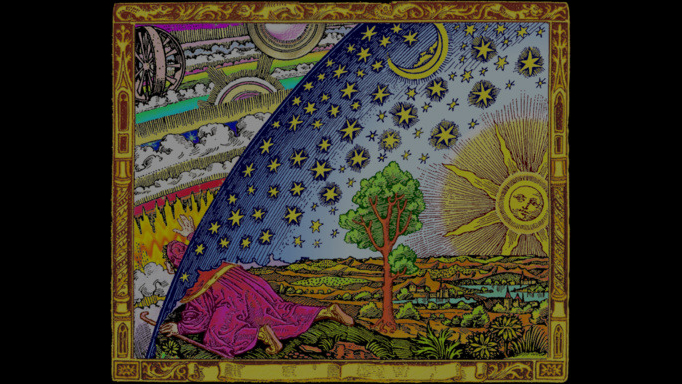
\includegraphics[height=\paperheight]{multiverse-faded-169}\end{minipage}}
\begin{frame}[c]
  \centering
  \color{white}

  \bigskip
  \bigskip
  \bigskip
  \bigskip

  \scriptsize
  \textit{-- an invitation --}

  \setbeamercolor{block body}{bg=black!100}
  \begin{minipage}{0.35\textwidth}
    \begin{block}{}
      \centering\normalsize\color{white}
      \hil{Constructive forcing}
    \end{block}
  \end{minipage}

  \bigskip
  \bigskip
  \bigskip
  \bigskip
  \bigskip
  \bigskip
  \bigskip

%  \colorbox{black!50}{Autumn school on} \\
%  \colorbox{black!50}{\emph{Proof and Computation}} \\
%  \colorbox{black!50}{in Herrsching} \\
%  \ \\
%  \colorbox{black!50}{September 20th to September 16th, 2023}
%
%  \colorbox{black!50}{Ingo Blechschmidt} \\
%  \par
\end{frame}}

\definecolor{mypurple}{RGB}{150,0,255}
\setbeamercolor{structure}{fg=mypurple}

\begin{frame}{}
  \begin{center}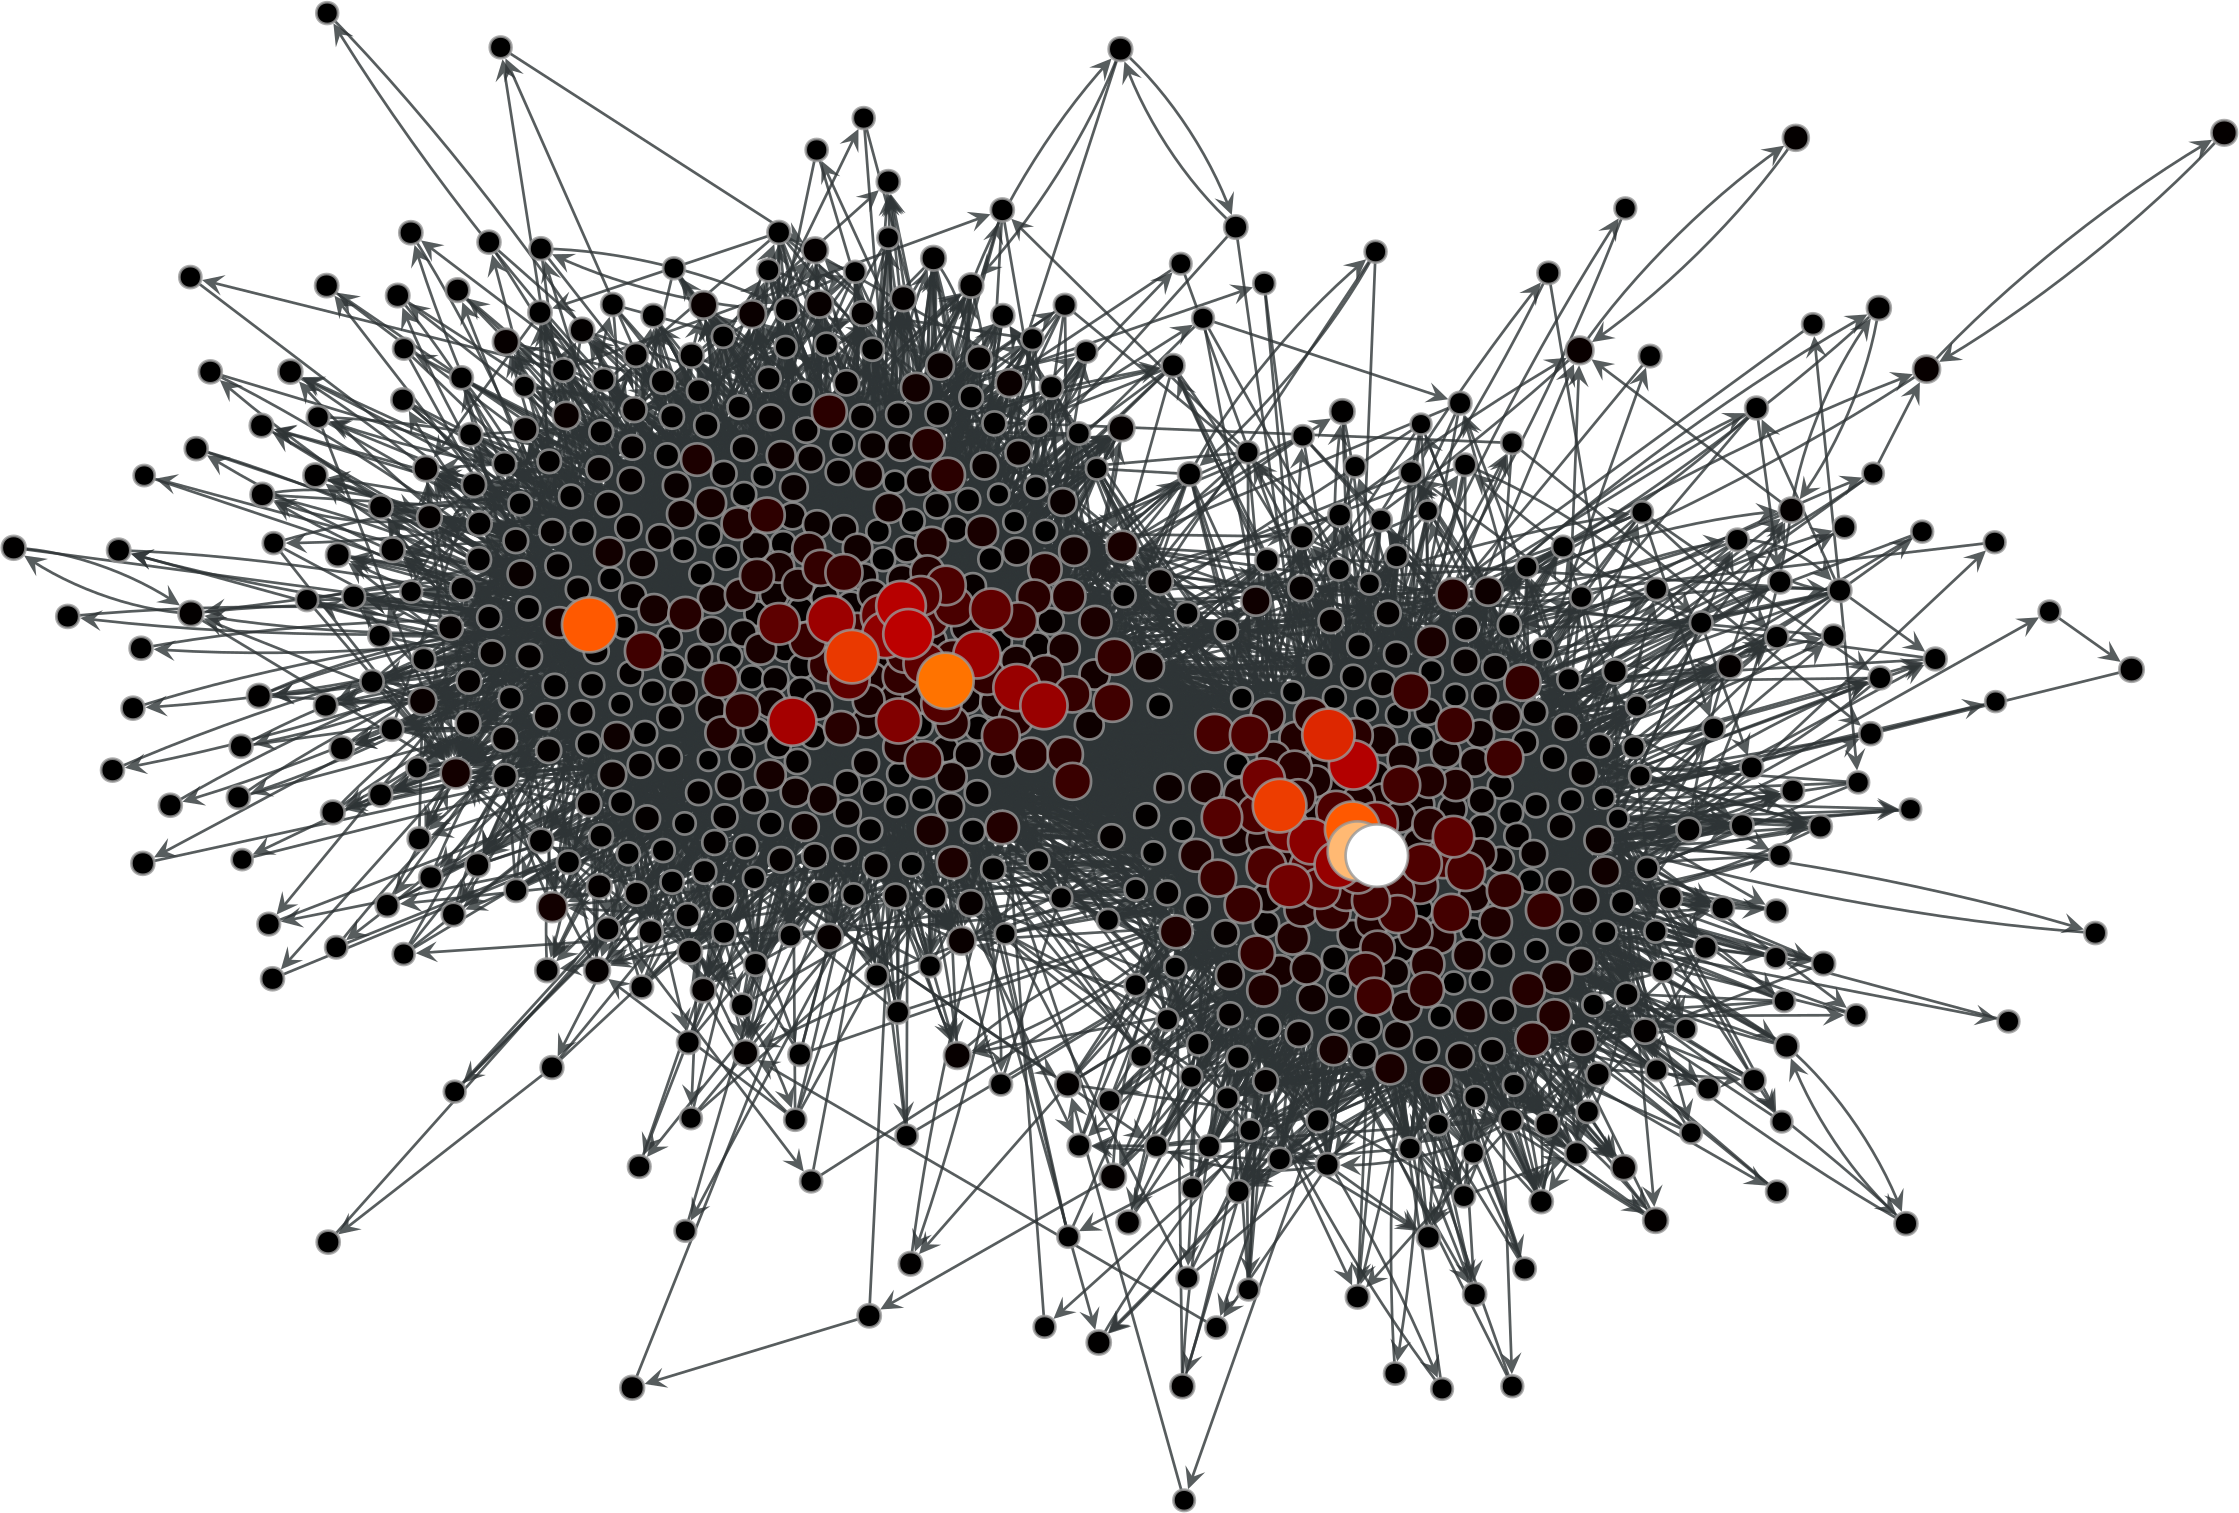
\includegraphics[width=0.2\textwidth]{eigenvector}\end{center}

  Let a continuous family of symmetric matrices be given:
  \[
  \begin{pmatrix}a_{11}(t)&\cdots&a_{1n}(t)\\\vdots&&\vdots\\a_{n1}(t)&\cdots&a_{nn}(t)\end{pmatrix}
  \]

  Then for every parameter value~$t \in \Omega$, classically there is

  \hil{$\blacktriangleright$} a full list of eigenvalues~$\lambda_1(t),\ldots,\lambda_n(t)$ and \\
  \hil{$\blacktriangleright$} an eigenvector basis~$(v_1(t),\ldots,v_n(t))$.
  \bigskip

  \begin{columns}[c]
    \begin{column}{0.01\textwidth}
      
\includegraphics[height=2.4em]{question-mark}
    \end{column}
    \begin{column}{0.9\textwidth}
      \mbox{Can locally the functions~$\lambda_i$ be chosen to be continuous?
      \only<2->{\hil{Yes.}}} \\
      How about the~$v_i$? \only<2->{\hil{No}\only<3->{, but \hil{yes} on a dense
      open subset of~$\Omega$.}}
    \end{column}
  \end{columns}
\end{frame}

% \begin{document}

\newcommand\ytl[2]{%
  \parbox[b]{4.5em}{\hfill{#1}~$\cdots\cdots$~}%
  \makebox[0pt][c]{\color{mypurple}$\bullet$}{\color{mypurple}\vrule}\quad%
  \parbox[c]{9.3cm}{\vspace{7pt}\raggedright#2\\[7pt]}%
  \\[-2.0pt]}
\begin{frame}{A brief timeline}
  \begin{columns}[t]
    \begin{column}{0.80\textwidth}
      \ytl{1878}{Cantor advances the \hil{continuum hypothesis}, the claim
      that~$2^{\aleph_0} = \aleph_1$.}
      \pause
      \ytl{1910s}{Zermelo--Fraenkel set theory emerges.}
      \pause
      \ytl{1920s}{Set theorists pursue additional axioms to
      settle~\textsc{ch} \\ (one way or another).}
      \pause
      \ytl{1938}{Gödel proves: If~\textsc{zfc} is consistent, so
      is~\textsc{zfc}+\textsc{ch}.}
      \pause
      \ytl{1963}{Cohen proves: If~\textsc{zfc} is consistent, so
      is~\textsc{zfc}+$\neg$\textsc{ch}.}
      \pause
      \ytl{2011}{Hamkins offers his paper on the \hil{multiverse position} in
      the philosophy of set theory.}
      \pause
      %arguing that the program of pursuing
      %additional axioms (while successful in many ways) is doomed to fail
      %to settle~\textsc{ch}.}
      \ytl{2016}{Oldenziel proposes to study the modal multiverse of parametrized
      mathematics.}
      \parbox[b]{4.5em}{\hfill\phantom{x}}\makebox[0pt][c]{\phantom{b}}{\color{mypurple}\vrule}\\[-6.5pt]
      \parbox[b]{4.5em}{\hfill\phantom{x}}\makebox[0pt][c]{\phantom{b}}{\color{mypurple}\vrule}\\[-6.5pt]
      \parbox[b]{4.5em}{\hfill\phantom{x}}\makebox[0pt][c]{\phantom{b}}{\color{mypurple}\vrule}\\[-6.5pt]
    \end{column}

    \begin{column}{0.20\textwidth}
      \pause
      \centering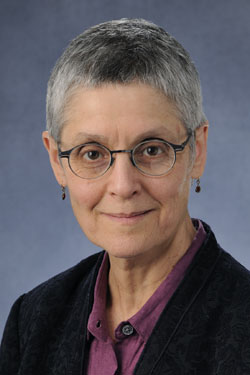
\includegraphics[width=\textwidth,valign=t]{roitman}

      \scriptsize Judith Roitman %(* 1945)
      \medskip

      \emph{Mainstream mathematics is beginning to see results using
      modern set theoretic techniques.}
    \end{column}
  \end{columns}
\end{frame}

{\usebackgroundtemplate{\begin{minipage}{\paperwidth}\vspace*{4.95cm}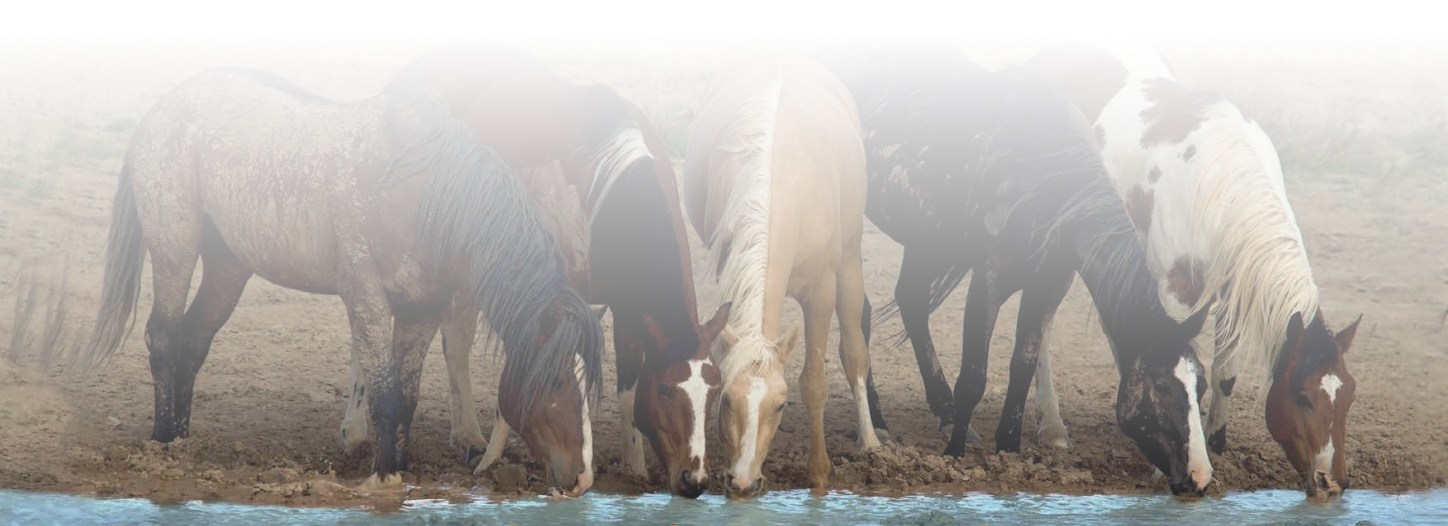
\includegraphics[width=\paperwidth]{topos-horses}\end{minipage}}
\begin{frame}{Constructive forcing}
  \medskip
  \begin{columns}[t]
    \begin{column}{0.40\textwidth}
      \quad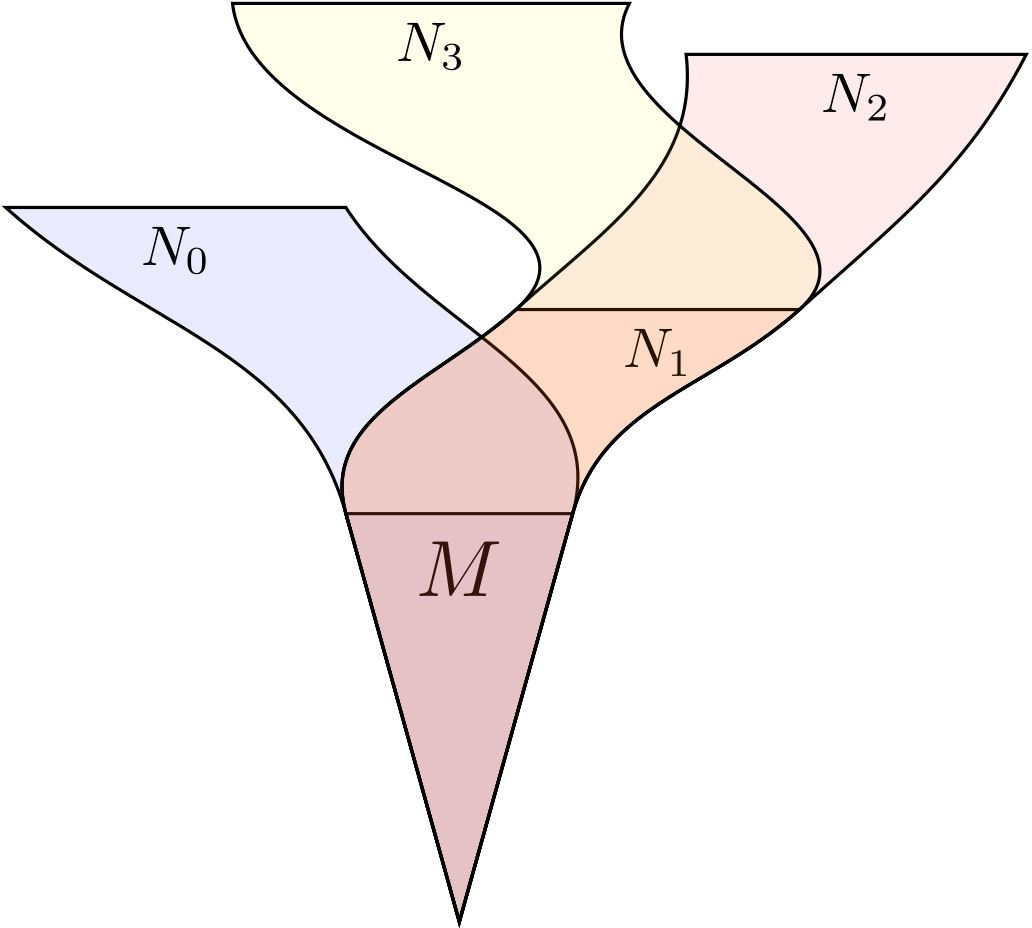
\includegraphics[width=0.8\textwidth,valign=t]{branching}
    \end{column}

    \begin{column}{0.75\textwidth}
      \hil{Extending the universe} in various ways, \\[0.7em]
      \pause
      \quad similarly how we can extend groups or rings, \\[0.7em]
      \pause
      \quad\quad in and for \hil{constructive mathematics} \\[0.7em]
      \pause
      \quad\quad\quad \hil{without} presupposing familiarity with \\[0.7em]
      \pause
      \quad\quad\quad\quad set theory, topos theory, or sheaves.
      \pause
    \end{column}
  \end{columns}

  \bigskip
  \bigskip

  \emph{Outline:}
  \vspace*{-0.5em}
  \begin{enumerate}
    \item What can forcing do for you?
    \item Forcing notions and Kripke--Joyal semantics
    \item Case studies in constructive algebra and combinatorics
  \end{enumerate}
\end{frame}}


\section{What can forcing do for you?}

\begin{frame}{What can forcing do for you?}
  \vspace*{-0.5em}

  \begin{columns}
    \begin{column}{0.45\textwidth}
      \begin{block}{1. Explore foundational possibility}
        There are forcing extensions with \\
        \textsc{ch}, $\neg$\textsc{ch}, \textsc{lem}, $\neg$\textsc{lem}, \ldots
      \end{block}
    \end{column}
    \pause

    \begin{column}{0.45\textwidth}
      \begin{block}{2. Demonstrate unprovability}
        The fundamental theorem of algebra is \hil{not constructively provable}
        as there is a forcing extension where \hil{it is false}.
      \end{block}
    \end{column}
  \end{columns}
  \pause
  \bigskip

  \begin{columns}
    \begin{column}{0.45\textwidth}
      \begin{block}{3. Harness convenient fictions}
        For every set, there is a forcing extension where it is
        \hil{countable}.
      \end{block}
    \end{column}
    \pause

    \begin{column}{0.45\textwidth}
      \begin{block}{4. Constructivize classical theories}
        A preorder~$X$ is well iff the \hil{generic sequence} $\NN \to X$ is
        good.
      \end{block}
    \end{column}
  \end{columns}
  \pause
  \bigskip

  \begin{columns}
    \begin{column}{0.45\textwidth}
      \begin{block}{5. Study parametric mathematics}
        Eigenvectors depend continuously on the parameter
        iff, in a suitable forcing extension, they merely exist.
      \end{block}
    \end{column}
    \pause

    \begin{column}{0.45\textwidth}
      \begin{block}{6. Develop synthetic accounts}
        \emph{As in the lectures by Matthias Hutzler.}
      \end{block}
    \end{column}
  \end{columns}
\end{frame}

{\usebackgroundtemplate{\begin{minipage}{\paperwidth}\vspace*{5.95cm}
\includegraphics[width=\paperwidth]{fr1}\end{minipage}}
\begin{frame}{Maximal ideals}
  \only<1-7>{\textbf{Thm.}
  Let~$M$ be a surjective matrix with more rows than columns over a
  ring~$A$. Then~$1 = 0$ in~$A$.

  \visible<2->{\emph{Proof.} \bad{Assume not.}}
  \visible<3->{Then there is~a \bad{maximal ideal} $\mmm$.}
  \visible<5->{The matrix is surjective over~$A/\mmm$.}
  \visible<6->{Since~$A/\mmm$ is a field, this is a contradiction to basic linear algebra.\qed}}

  \only<4-7>{\bigskip\par\centering\scalebox{0.9}{\centering\begin{tikzpicture}
    \node (0) at (0,1) {$(0) = \{0\}$};
    \node (1) at (0,5) {$(1) = \ZZ$};
    \node (2) at (-2,4) {$(2)$};
    \node [right of=2] (3) {$(3)$};
    \node [below of=2] (4) {$(4)$};
    \node [below of=2, xshift=0.7cm] (6) {$(6)$};
    \node [right of=3] (5) {$(5)$};
    \node [right of=5] (7) {$(7)$};
    \node [right of=7] (7d) {$\ldots$\phantom{(}};
    \node [right of=7d, xshift=3cm, yshift=-2cm] (max)
    {\vbox{\small{\it maximal among the proper ideals} \\ \medskip \hspace*{-6.75em}\textbullet \quad $\neg(1 \in
    \mmm)$ \\ \medskip \textbullet \quad $x \in \mmm \quad\vee\quad 1 \in \mmm + (x)$}};
    \node [below of=4] (8) {$(8)$};
    \node [right of=8, xshift=3cm] (8d) {$\ldots$};
    \draw (0) -- (8);
    \draw (0) -- (8d);
    \draw (0) -- (6);
    \draw (2) -- (1);
    \draw (3) -- (1);
    \draw (5) -- (1);
    \draw (7) -- (1);
    \draw (7d) -- (1);
    \draw (4) -- (2);
    \draw (8) -- (4);
    \draw (6) -- (2);
    \draw (6) -- (3);
    \draw [mypurple!30, thick, shorten <=-2pt, shorten >=-2pt, ->] (max) to [out=120, in=-30] (7d);
    \begin{pgfonlayer}{background}
      \draw[decorate, very thick, draw=mypurple!30]
        ($(2.south west) + (8pt, 0)$) arc(270:180:8pt) --
        ($(2.north west) + (0, -8pt)$) arc(180:90:8pt) --
        ($(7d.north east) + (-8pt, 0)$) arc(90:0:8pt) --
        ($(7d.south east) + (0, 8pt)$) arc(0:-90:8pt) --
        cycle;
    \end{pgfonlayer}
  \end{tikzpicture}\par}\par}

  \pause
  \pause
  \pause
  \pause
  \pause
  \pause
  \medskip
  \raggedright

  Let~$A$ be a ring. \emph{Does there exist a maximal ideal~$\mmm \subseteq A$?}
  \pause
  \begin{enumerate}
    \item \good{Yes}, if \bad{Zorn's lemma} is available.
    \bigskip
    \pause

    \item \good{Yes}, if~$A$ is countable and membership of finitely generated ideals is decidable:
    {\footnotesize
    Let~$A = \{ x_0, x_1, \ldots \}$. Then set:
    \begin{align*}
      \mmm_0 &\defeq \{ 0 \}, &
      \mmm_{n+1} &\defeq \begin{cases}
        \mmm_n + (x_n), & \text{if $1 \not\in \mmm_n + (x_n)$}, {\qquad\quad\quad\!\!}\\
        \mmm_n, & \text{else.}
      \end{cases}
    \end{align*}}
    \pause

    \item \good{Yes}, if~$A$ is countable (irrespective of membership decidability):
    {\footnotesize\begin{align*}
      \mmm_0 &\defeq \{ 0 \}, &
      \mmm_{n+1} &\defeq \mmm_n + (\underbrace{\{ x \in A \,|\, x = x_n \wedge
        1 \not\in \mmm_n + (x_n) \}}_{\text{a certain subsingleton set}})
    \end{align*}}
    \vspace*{3.5em}
    \visible<11>{{
      \centering
      \raisebox{0pt}[0pt][0pt]{
        \hspace*{2.5em}
        \scalebox{0.9}{\begin{tikzpicture}
          \node (inner) at (17.3mm,-20mm) {\textit{``a bad joke''}};
          \path (0,0) pic{laurel-wreath};
        \end{tikzpicture}}
        \hspace*{-3em}
        \scalebox{0.9}{\begin{tikzpicture}
          \node (inner) at (17.5mm,-18mm) {\vbox{\small\centering\textit{``non- \\informative''}}};
          \path (0,0) pic{laurel-wreath};
        \end{tikzpicture}}
      }
      \par
    }}
    \pause
    \pause
    \vspace*{-3.5em}

    \item In the general case: \bad{No}\pause, but \good{yes} in a \emph{suitable forcing extension}\pause, and \\
    \emph{first-order consequences} of its existence there \good{do hold} in
    the base universe.
  \end{enumerate}
\end{frame}

\begin{frame}{Maximal ideals}
  \textbf{Thm.}
  Let~$M$ be a surjective matrix with more rows than columns over a
  ring~$A$. Then~$1 = 0$ in~$A$.

  \emph{Proof.} (special case) Write~$M = \left(\begin{smallmatrix}x\\y\end{smallmatrix}\right)$. By surjectivity,
  have~$u, v \in A$ with
  \[
    u \left(\begin{smallmatrix}x\\y\end{smallmatrix}\right) = \left(\begin{smallmatrix}1\\0\end{smallmatrix}\right)
    \quad\text{and}\quad
    v \left(\begin{smallmatrix}x\\y\end{smallmatrix}\right) = \left(\begin{smallmatrix}0\\1\end{smallmatrix}\right).
  \]
  Hence
  $
    1 = (vy) (ux) = (uy) (vx) = 0
  $. \qed
\end{frame}}

{\usebackgroundtemplate{\begin{minipage}{\paperwidth}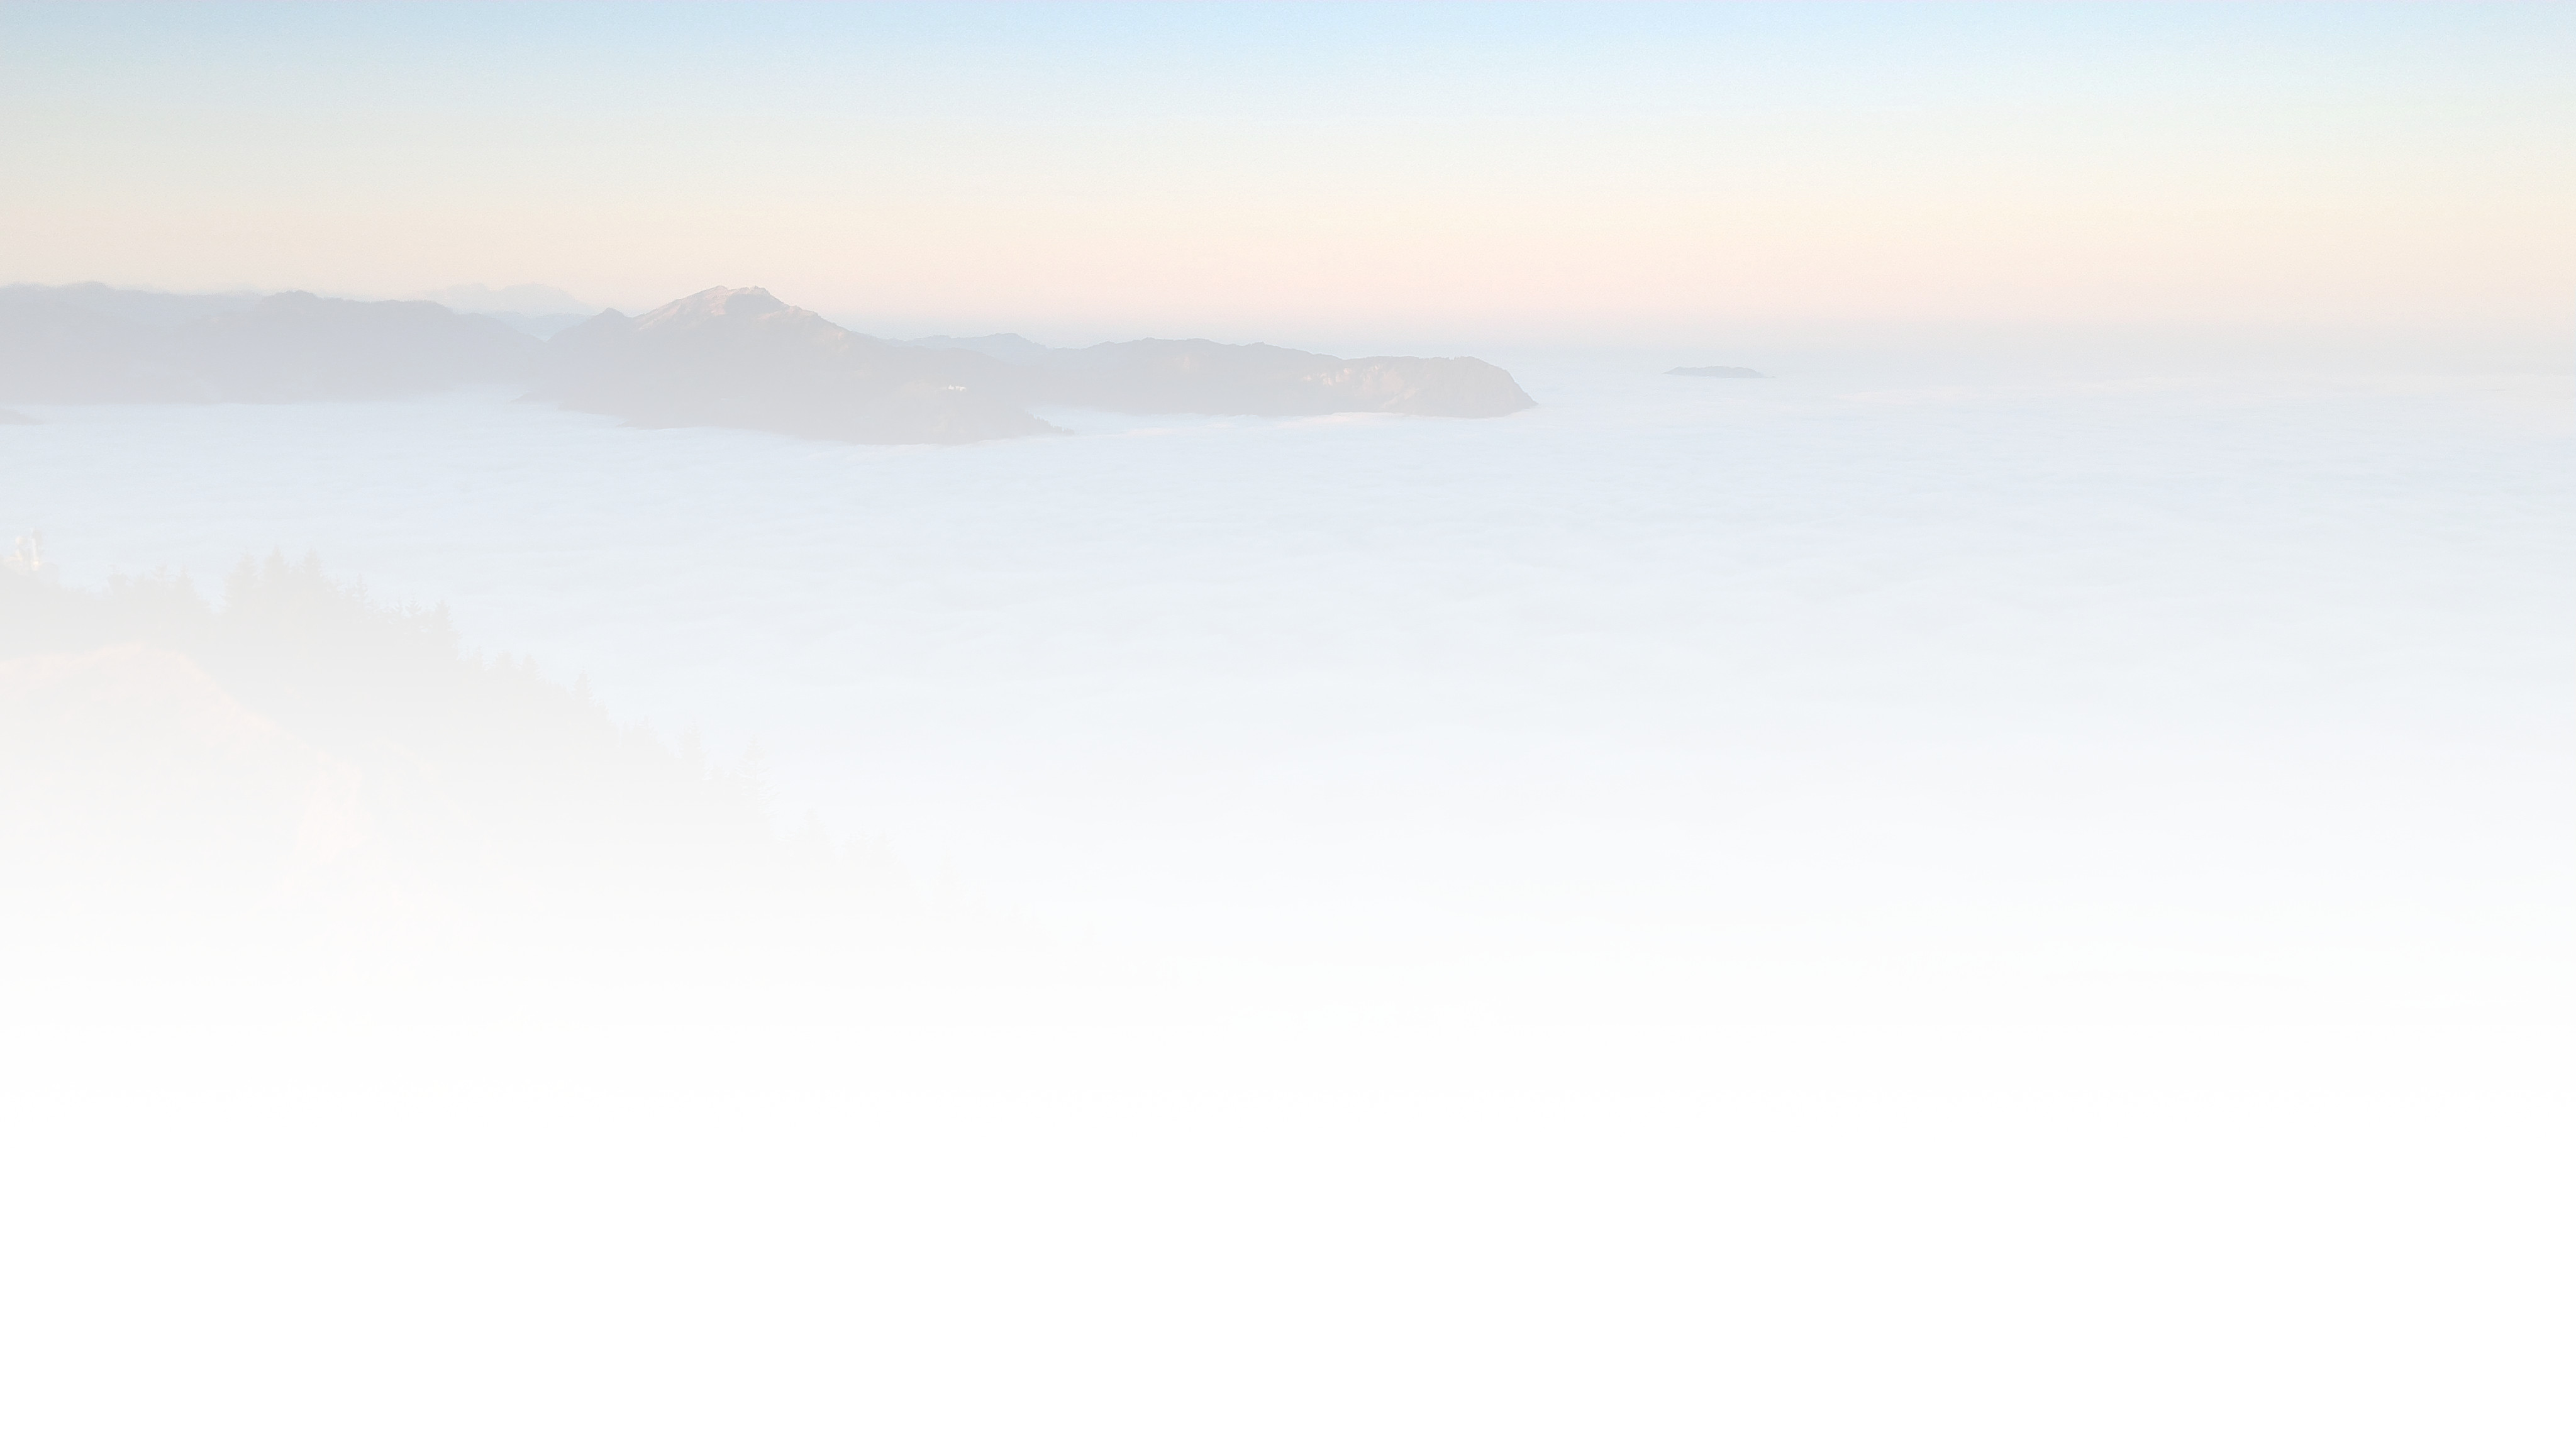
\includegraphics[height=\paperheight]{sea-of-clouds-2}\end{minipage}}
\begin{frame}{Infinite data}
  \vspace*{-1em}
  \[ \astikznodetransparentlycircled{xm}{7}\!,
    \quad \astikznodetransparentlycircled{x0}{4}\!,
    \quad \only<1-2>{\astikznodetransparentlycircled{t1}{3}}\only<3->{\astikznodecircled{t1}{mypurple}{3}}\!,
    \quad \only<1>{\ldots}\pause \astikznodetransparentlycircled{x1}{1}\!,
    \quad \only<2>{\ldots}\pause \astikznodecircled{t2}{mypurple}{8}\!,
    \quad \only<3>{\ldots} \visible<4->{\astikznodetransparentlycircled{x2}{2}\!,}
    \quad \only<4->{\ldots} \]
  {\centering\begin{tikzpicture}[remember picture,overlay]
    \node[draw=mypurple, circle, thick, inner sep=0.1em] (t3) {\scriptsize$\leq$};
    \path[draw=mypurple,thick]
      (t1)
      to [out=-90, in=180] (t3)
      to [out=0, in=-90] (t2);
  \end{tikzpicture}\par}
  \medskip
  \pause

  \textbf{Thm.} Every sequence~$\alpha : \NN \to \NN$ is \hil{good} in that
  there exist~$i < j$ with~$\alpha(i) \leq \alpha(j)$.
  \pause

  \emph{Proof.} \emph{(offensive?)} By~\badbox{\textsc{lem}}, there is a
  minimum~$\alpha(i)$.
  Set~$j \defeq i + 1$. \qed\par
  \pause
  \medskip

  \textbf{Def.} A preorder~$X$ is \hil{well\only<9->{$^\star$}} iff every sequence~$\NN \to X$ is good.

  \textbf{Examples.} $(\NN,{\leq}),\ \
  \color{white}\only<7->{\color{red!90}}\astikznode{onlyclass}{$\underbrace{\color{black}X \times Y,\ \ X^*,\ \ \mathrm{Tree}(X)}_{\text{\visible<7->{\bad{only classically}}}}$}$.
  \pause
  \pause
  \medskip

  \begin{tikzpicture}[remember picture,overlay]
    \node[thick, fill=black, rectangle, inner sep=0.3em, right=2em of onlyclass] (moral) {
      \begin{minipage}{6cm}
        \begin{columns}
          \begin{column}{0.15\textwidth}
            \hspace*{1.0em}\color{white}\dbend
          \end{column}
          \begin{column}{0.95\textwidth}
            \color{white}\footnotesize
            \it Don't quantify over points of spaces which might not have enough.
          \end{column}
        \end{columns}
      \end{minipage}
    };
    \path[draw=red!90,thick,-stealth]
      (moral) to
      [out=180, in=-00] (onlyclass.east);
  \end{tikzpicture}
  \pause

  \textbf{Def.} A preorder is \hil{well} iff any of the following equivalent
  conditions hold:
  \begin{enumerate}
    \item The \hil{generic sequence} $\NN \to X$ is good.
    \pause
    \item Every sequence $\NN \to X$ \hil{in every forcing extension} is good.
    \pause
    \item There is a \hil{well-founded tree} witnessing universal goodness.
  \end{enumerate}

%  $\mathsf{Good}\,[\sigma_1,\ldots,\sigma_n] \defeqv (\exists(i < j)\_ \sigma_i \leq \sigma_j)$.
%  \textbf{Def.} For a predicate~$P$ on finite lists over a set~$X$, inductively
%  define:
%  \[
%    \infer{P \,|\, \sigma}{P\sigma}
%    \qquad
%    \infer{P \,|\, \sigma}{\forall(x \in X)\_\ P \,|\, \sigma x}
%  \]
%
%  \textbf{Def.} A preorder is \hil{well} iff~$\mathsf{Good} \,|\, [\,]$, where
%  $\mathsf{Good}\,[\sigma_1,\ldots,\sigma_n] \defeqv (\exists(i < j)\_ \sigma_i \leq \sigma_j)$.
\end{frame}}


\section{Basics of forcing}

\begin{frame}{Ingredients for forcing}
  To construct a forcing extension, we require:
  \begin{enumerate}
    \item a base universe~$V$
    \item a preorder~$L$ of \hil{forcing conditions} in~$V$\!,
    pictured as \hil{finite approximations}

    (\emph{convention:} $\tau \preccurlyeq \sigma$ means that~$\tau$ is a
    better finite approximation than~$\sigma$)
    \item a \hil{covering system} governing how finite approximations evolve to
    better ones

    (for each~$\sigma \in L$, a set~$\Cov(\sigma) \subseteq
    P({\downarrow}\sigma)$, with a simulation condition)
  \end{enumerate}
  In the forcing extension~$V^\nabla$, there will then be a \hil{generic filter} (ideal
  object).
  \pause

  \vspace*{-1em}
  \begin{columns}
    \begin{column}{0.49\textwidth}
      \small
      \begin{block}{For the generic surjection~$\NN \twoheadrightarrow X$}
        \justifying
        Use \hil{finite lists}~$\sigma \in X^*$ as forcing conditions,
        where $\tau \preccurlyeq \sigma$ iff~$\sigma$ is an initial segment of~$\tau$,
        and be prepared to grow~$\sigma$ to \ldots
        \footnotesize
        \begin{enumerate}
          \item[(a)] one of~$\{ \sigma x \,|\, x \in X \}$, to make~$\sigma$ more defined
          \item[(b)] one of~$\{ \sigma \tau \,|\, \tau \in X^*, a \in
          \sigma\tau \}$, for any~$a \in X$, to make~$\sigma$ more surjective
        \end{enumerate}
      \end{block}
    \end{column}
    \pause

    \begin{column}{0.45\textwidth}
      \small
      \begin{block}{For the generic prime ideal of a ring~$A$}
        \justifying
        Use \hil{f.g.\@ ideals} as forcing conditions, where $\bbb \preccurlyeq
        \aaa$ iff~$\bbb \supseteq \aaa$, and be prepared to grow~$\aaa$ to \ldots
        \footnotesize
        \begin{enumerate}
          \item[(a)] one of~$\emptyset$, if~$1 \in \aaa$, to make~$\aaa$ more proper
          \item[(b)] one of~$\{ \aaa+(x), \aaa+(y) \}$, if~$xy \in \aaa$, to
          make~$\aaa$ more prime
        \end{enumerate}
      \end{block}
    \end{column}
  \end{columns}
\end{frame}

\begin{frame}{The eventually monad}
  Let~$L$ be a forcing notion.

  Let~$P$ be a monotone predicate on~$L$
  (if $\tau \preccurlyeq \sigma$, then $P\sigma \Rightarrow P\tau$). \\
  For instance, in the case~$L = X^*$:
  \begin{itemize}
    \item $\mathsf{Repeats}\, x_0\ldots x_{n-1} \defeqv \exists i\_ \exists j\_ i < j \wedge x_i = x_j$
    \item $\mathsf{Good}\, \,\,\,\,\,\,x_0\ldots x_{n-1} \defeqv \exists i\_ \exists j\_ i < j \wedge x_i \leq x_j$
    \quad (for some preorder~$\leq$ on~$X$)
  \end{itemize}
  \pause

  We then define~``\hil{$P \mid \sigma$}'' (``$P$ bars~$\sigma$'') inductively by the following clauses:
  \begin{enumerate}
    \item If~$P\sigma$, then~$P \mid \sigma$.
    \item If~$P \mid \tau$ for all~$\tau \in R$, where~$R$ is some covering
    of~$\sigma$, then~$P \mid \sigma$.
  \end{enumerate}
  So~$P \mid \sigma$ expresses in a \hil{direct inductive fashion}:
  \[ \text{``No matter
  how~$\sigma$ evolves to a better approximation~$\tau$, eventually~$P\tau$
  will hold.''} \]

  \pause
  We use quantifier-like notation: ``$\nabla(\tau \preccurlyeq \sigma)\_
  P\tau$'' means ``$P \mid \sigma$''.
\end{frame}
% BOARD:
% - examples for P | σ
% - abuse of notation

\begin{frame}{Proof translations}
  \textbf{Thm.} Every~\textsc{iqc}-proof remains correct, with at most a
  polynomial increase in length, if throughout we
  replace
  \[\begin{array}{rcl@{\quad\text{where}\quad}rcl}
    \exists & \leadsto & \exists_\mathrm{class},
    & \exists_\mathrm{class} &\defeqv& \neg\neg\exists, \\
    \vee & \leadsto & \vee_\mathrm{class},
    & \alpha \vee_\mathrm{class} \beta &\defeqv& \neg\neg(\alpha \vee \beta), \\
    = & \leadsto & =_\mathrm{class},
    & s =_\mathrm{class} t &\defeqv& \neg\neg(s = t).
  \end{array} \]
  \pause

  \begin{columns}[c]
    \begin{column}{0.01\textwidth}
      
\includegraphics[height=2.4em]{sheafification-man-2}
    \end{column}
    \quad
    \begin{column}{0.9\textwidth}
      \hil{When we say:}\ \ some statement ``holds in~$V^{\neg\neg}$'', \\
      \makesamewidth[l]{\hil{When we say:}}{\hil{we mean:}}\ \ its translation holds in~$V$.
    \end{column}
  \end{columns}
  \bigskip

  Similarly for arbitrary forcing extensions~$V^\nabla$, ``just with~$\nabla$
  instead of~$\neg\neg$''.
  \bigskip

  \pause
  \textbf{Ex.} As~$\neg\neg(\varphi \vee \neg\varphi)$ is a theorem
  of~\textsc{iqc}, the law of excluded middle holds in~$V^{\neg\neg}$.
\end{frame}

% \begin{document}

\newcommand{\defeqvi}{\quad iff\quad}
\begin{frame}{The $\nabla$-translation}
  \small
  \only<1>{For bounded first-order formulas over the (large) first-order signature which has
  \begin{enumerate}
    \scriptsize
    \item one sort~$\underline{X}$ for each set~$X$ in the base universe,
    \\[-1.2em]
    \item one~$n$-ary function symbol~$\underline{f} : \underline{X_1} \times
    \cdots \times \underline{X_n} \to \underline{Y}$ for each map~$f : X_1 \times
    \cdots \times X_n \to Y$,
    \\[-1.2em]
    \item one~$n$-ary relation symbol~$\underline{R} \hookrightarrow
    \underline{X_1} \times \cdots \times \underline{X_n}$ for each relation~$R
    \subseteq X_1 \times \cdots \times X_n$, and
    \\[-1.2em]
    \item an additional unary relation symbol~$G \hookrightarrow \underline{L}$
    (for the \emph{generic filter} of~$L$),
  \end{enumerate}
  we recursively define:}
  \scriptsize
  \begin{tabbing}
    \quad \= $\sigma \forces \forces \forall(x\?\underline{X})\_ \varphi$ \=
    \defeqvi $\textcolor{gray}{\forall(\tau \preccurlyeq \sigma)\_}\
    \forall(x_0 \in X)\_ \tau \forces \varphi[\underline{x_0}/x]$.\qquad\quad \=
    $\sigma \forces \exists(x\?\underline{X})\_ \varphi$
    \= $\sigma \forces \underline{R}(\underline{s_1},\ldots,\underline{s_n})$ \= \defeqvi $s = t$. \= \kill

    \> $\sigma \forces s = t$
    \> \defeqvi $\nabla \sigma\_ \llbracket s \rrbracket = \llbracket t \rrbracket$.
    \> $\sigma \forces \underline{R}(s_1,\ldots,s_n)$
    \> \defeqvi $\nabla\sigma\_ R(\llbracket s_1 \rrbracket,\ldots,\llbracket s_n \rrbracket)$. \\[0.3em]

    \> $\sigma \forces \varphi \Rightarrow \psi$
    \> \defeqvi $\textcolor{gray}{\forall(\tau \preccurlyeq \sigma)\_}\ (\tau \forces \varphi) \Rightarrow
    (\tau \forces \psi)$.
    \> $\sigma \forces G\tau$
    \> \defeqvi $\nabla\sigma\_ \sigma \preccurlyeq \llbracket\tau\rrbracket$. \\[0.3em]

    \> $\sigma \forces \top$ \> \defeqvi $\top$.
    \> $\sigma \forces \bot$ \> \defeqvi $\hil{$\nabla\sigma\_$}\ \bot$ \\[0.3em]

    \> $\sigma \forces \varphi \wedge \psi$
    \> \defeqvi $(\sigma \forces \varphi) \wedge (\sigma \forces \psi)$.
    \> $\sigma \forces \varphi \vee \psi$
    \> \defeqvi $\hil{$\nabla\sigma\_$}\ (\sigma \forces \varphi) \vee (\sigma \forces \psi)$. \\[0.3em]

    \> $\sigma \forces \forall(x\?\underline{X})\_ \varphi$
    \> \defeqvi $\textcolor{gray}{\forall(\tau \preccurlyeq \sigma)\_}\ \forall(x_0 \in X)\_ \tau \forces
    \varphi[\underline{x_0}/x]$.
    \> $\sigma \forces \exists(x\?\underline{X})\_ \varphi$
    \> \defeqvi $\hil{$\nabla\sigma\_$}\ \exists(x_0 \in X)\_ \sigma \forces \varphi[\underline{x_0}/x]$.
  \end{tabbing}
  \small
  \only<1>{Finally, we say that~$\varphi$ ``holds in~$V^\nabla$'' iff for all~$\sigma
  \in L$, $\sigma \forces \varphi$.}

  \footnotesize
  \begin{tabular}{@{}lp{0.27\textwidth}p{0.48\textwidth}}
    \toprule
    forcing notion & statement about~$V^\nabla$ & external meaning \\
    \midrule
    surjection $\NN \twoheadrightarrow X$ &
    ``the gen.\@ surj.\@ is surjective'' &
    $\forall(a{\in}X)\_ \forall(\sigma{\in}X^*)\_ \nabla(\tau{\preccurlyeq}\sigma)\_ \exists(n{\in}\NN)\_ \tau[n] = a$. \\[0.5em]
    \pause

    map $\NN \to X$ &
    ``the gen.\@ sequence is good'' &
    $\mathsf{Good} \mid [\,]$. \\[0.5em]

    frame of opens &
    ``every complex number has a square root'' &
    For every open~$U \subseteq X$ and every cont.\@
    function $f : U \to \CC$, there is an open covering $U = \bigcup_i U_i$ such
    that for each index~$i$, there is a cont.\@ function $g : U_i \to \CC$
    such that~$g^2 = f$. \\[4.5em]

    Zariski &
    ``$x \neq 0 \Rightarrow \text{$x$ inv.}$'' &
    if the only f.p.\@ $k$-algebra in which~$x = 0$ is the zero algebra,
    then~$x$ is invertible in~$k$
  \end{tabular}
\end{frame}

\begin{frame}{Formalities}
  \small
  \textbf{Def.} A \hil{forcing notion} consists of
  a preorder~$L$ of \hil{forcing conditions}, and
  for every~$\sigma \in L$, a set~$\Cov(\sigma) \subseteq
  P({\downarrow}\sigma)$ of \hil{coverings} of~$\sigma$
  such that: If~$\tau \preccurlyeq \sigma$ and~$R \in \Cov(\sigma)$, there
  should be a covering~$S \in \Cov(\tau)$ such that~$S \subseteq
  {\downarrow}R$.
  \bigskip

  {\centering\footnotesize\begin{tabular}{llll}
    \toprule
    & preorder~$L$ & coverings of an element~$\sigma \in L$ & filters of~$L$ \\
    \midrule
    \normalnumber{1} & $X^*$ & $\{ \sigma x \,|\, x \in X \}$ & maps~$\NN \to X$ \\
    \normalnumber{2} & $X^*$ & $\{ \sigma x \,|\, x \in X \}$,\ \ $\{ \sigma\tau \,|\, \tau \in X^*, a \in \sigma\tau \}$ for each~$a \in X$ & surjections~$\NN \twoheadrightarrow X$ \\
    \normalnumber{3} & f.g. ideals & --- & ideals \\
    \normalnumber{4} & f.g. ideals & $\{ \sigma+(a), \sigma+(b) \}$ for each~$ab \in \sigma$,\ \ $\{\}$ if~$1 \in \sigma$ & prime ideals \\
    \normalnumber{5} & opens & $\mathcal{U}$ such that~$\sigma = \bigcup \mathcal{U}$ & points \\
    \normalnumber{6} & $\{\star\}$ & $\{ \star \,|\, \varphi \} \cup \{ \star \,|\, \neg\varphi \}$ &
    witnesses of~\textsc{lem}
    \\
    \bottomrule
  \end{tabular}\par}
  \bigskip

  \textbf{Def.} A \emph{filter} of a forcing notion~$(L,\mathrm{Cov})$
  is a subset~$F \subseteq L$ such that
  \vspace*{-0.4em}
  \begin{enumerate}
    \scriptsize
    \item $F$ is upward-closed: if~$\tau \preccurlyeq \sigma$ and if~$\tau \in F$, then~$\sigma \in F$; \\[-3.0em]
    \item $F$ is downward-directed: $F$ is inhabited, and if~$\alpha,\beta \in F$,
    then there is a common refinement~$\sigma \preccurlyeq \alpha,\beta$ such
    that~$\sigma \in F$; and \\[-2.0em]
    \item $F$ splits the covering system: if~$\sigma \in F$ and~$R \in
    \Cov(\sigma)$, then~$\tau \in F$ for some~$\tau \in R$.
  \end{enumerate}
\end{frame}

\addtocounter{framenumber}{-1}

\end{document}

- Judith Roitman
- Proof and Computation

- What can forcing do for you?
  - Exploring the range of foundational possibility: CH, ¬CH, FTA, ...
  - Eigenvalues
  - Generic sequence
  - Generic surjection
  - Matthias
  - "Harness the flexibility of parametric mathematics in an accessible way."

Overloading

1. Eigenvalues
2. Generic surjection
3. Generic sequence
4. FTA

Extending the universe in various ways,

similarly how we can extend groups or rings,

in the context of and for the purposes of constructive mathematics

without requiring knowledge of

set theory, topos theory, category theory, sheaves.


Dominique Duval



Forschungsfrage: Klassische Basen sind ja schon ziemlich maximal in dem Sinn,
als dass etwa der Raum der Funktionen ℕ → ℕ genügend Punkte hat. Wie wäre es,
in einer Welt zu arbeiten, in der auch der Raum der Surjektionen ℕ → X genügend
Punkte hat?


Fun:
- Modale Dinge
- structure sheaf A~, field property etc. (like in redcom slides), generic freeness
- nongeometric surprises


\newcommand{\Good}{\mathsf{Good}}
\newcommand{\vinfer}[2]{\left.#1\quad\middle|\quad\begin{array}{l}#2\end{array}\right.}
\begin{frame}[plain]
  \scriptsize
  \[
    \renewcommand{\arraystretch}{1.3}
    \vinfer{\Good \mid [\,]}{
      \vinfer{\Good \mid 0}{
        \vinfer{\Good \mid 00}{\Good\ 00} \\[1em]
        \vinfer{\Good \mid 01}{\Good\ 01} \\[1em]
        \vinfer{\Good \mid 02}{\Good\ 02} \\
        \vdots
      } \\[1em]
      \ \\[0.5em]
      \vinfer{\Good \mid 1}{
        \vinfer{\Good \mid 10}{
          \vinfer{\Good \mid 100}{\Good\ 100} \\[1em]
          \vinfer{\Good \mid 101}{\Good\ 101} \\[1em]
          \vinfer{\Good \mid 102}{\Good\ 102} \\
          \vdots
        } \\[1em]
        \vinfer{\Good \mid 11}{\Good\ 11} \\[1em]
        \vinfer{\Good \mid 12}{\Good\ 12} \\[1em]
        \vdots
      } \\[1em]
      \ \\[0.5em]
      \vinfer{\Good \mid 2}{} \\[1em]
      \vdots
    }
  \]
\end{frame}
